\documentclass[crop,tikz]{standalone}% 'crop' is the default for v1.0, before it was 'preview'
%\usetikzlibrary{...}% tikz package already loaded by 'tikz' option
\usetikzlibrary{shapes,snakes}
\usepackage{amsmath}
\begin{document}
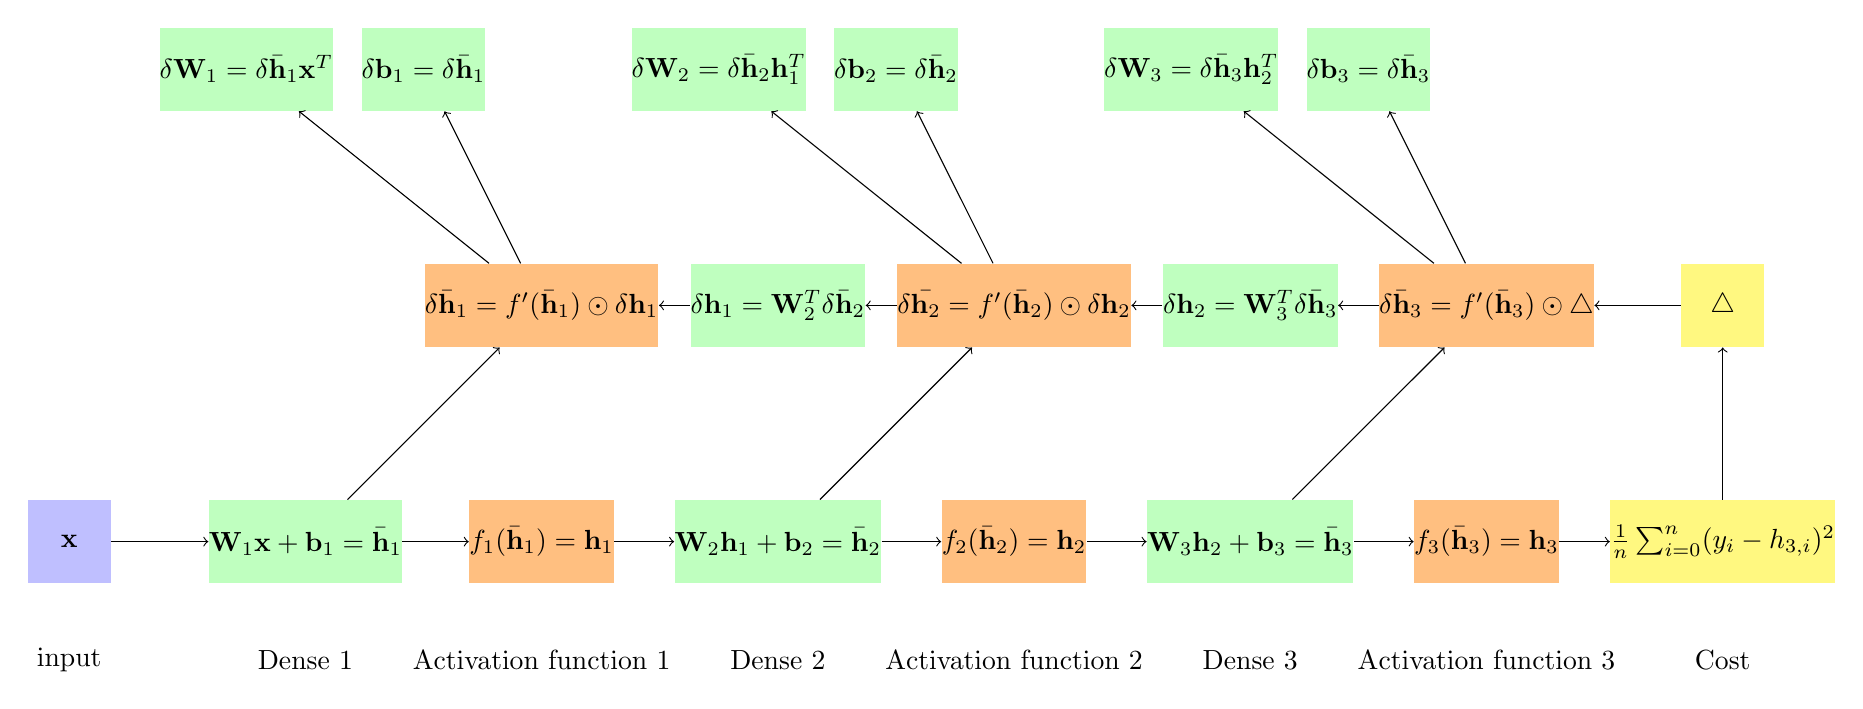
\begin{tikzpicture}

\def\vertspace{1.5cm}
\def\horispace{3.0cm}


\tikzstyle{input}=[rectangle,fill=blue!25,minimum size=30pt,inner sep=0pt]
\tikzstyle{neuron}=[rectangle,fill=green!25,minimum size=30pt,inner sep=0pt]
\tikzstyle{activation}=[neuron, fill=orange!50];
\tikzstyle{output}=[neuron, fill=yellow!50];

%inputs
\node (in) at (\horispace,-1*\vertspace) {input};
\node[input] (x1) at (\horispace,0*\vertspace) {$\mathbf{x}$};

%weights
\node[neuron] (n1) at (2*\horispace, 0*\vertspace) {$\mathbf{W}_1 \mathbf{x} + \mathbf{b}_1 = \bar{\mathbf{h}}_1$};
\node[activation] (a1) at (3*\horispace,0*\vertspace) {$f_1(\bar{\mathbf{h}}_1) = \mathbf{h}_1$};
\node (n1label) at (2*\horispace,-1*\vertspace) {Dense 1};
\node (a1label) at (3*\horispace,-1*\vertspace) {Activation function 1};


\node[neuron] (n2) at (4*\horispace, 0*\vertspace) {$\mathbf{W}_2 \mathbf{h}_1 + \mathbf{b}_2 = \bar{\mathbf{h}}_2$};
\node[activation] (a2) at (5*\horispace,0*\vertspace) {$f_2(\bar{\mathbf{h}}_2) = \mathbf{h}_2$};
\node (n2label) at (4*\horispace,-1*\vertspace) {Dense 2};
\node (a2label) at (5*\horispace,-1*\vertspace) {Activation function 2};


\node[neuron] (n3) at (6*\horispace, 0*\vertspace) {$\mathbf{W}_3 \mathbf{h}_2 + \mathbf{b}_3 = \bar{\mathbf{h}}_3$};
\node[activation] (a3) at (7*\horispace,0*\vertspace) {$f_3(\bar{\mathbf{h}}_3) = \mathbf{h}_3$};
\node (n3label) at (6*\horispace,-1*\vertspace) {Dense 3};
\node (a3label) at (7*\horispace,-1*\vertspace) {Activation function 3};

\node[output] (cost) at (8*\horispace, 0*\vertspace) {$\frac{1}{n}\sum_{i=0}^n (y_i - h_{3,i})^2$}; 
\node (costlabel) at (8*\horispace,-1*\vertspace) {Cost};

\draw[->] (x1) -- (n1);
\draw[->] (n1) -- (a1);
\draw[->] (a1) -- (n2);
\draw[->] (n2) -- (a2);
\draw[->] (a2) -- (n3);
\draw[->] (n3) -- (a3);
\draw[->] (a3) -- (cost);

% backprop
\node[output](deltacost) at (8*\horispace, 2*\vertspace) {$\triangle$};
\draw[->] (cost) -- (deltacost);
\node[activation] (da3) at (7*\horispace, 2*\vertspace) {$\delta \bar{\mathbf{h}}_3 = f'(\bar{\mathbf{h}}_3) \odot \triangle$};
\node[neuron] (dn3) at (6*\horispace, 2*\vertspace) {$\delta \mathbf{h}_2 = \mathbf{W}_3^T \delta \bar{\mathbf{h}}_3$};
\node[activation] (da2) at (5*\horispace, 2*\vertspace) {$\delta \bar{\mathbf{h}_2} = f'(\bar{\mathbf{h}}_2) \odot \delta \mathbf{h}_2$};
\node[neuron] (dn2) at (4*\horispace, 2*\vertspace) {$\delta \mathbf{h}_1 = \mathbf{W}_2^T \delta \bar{\mathbf{h}}_2$};
\node[activation] (da1) at (3*\horispace, 2*\vertspace) {$\delta \bar{\mathbf{h}}_1 = f'(\bar{\mathbf{h}}_1) \odot \delta \mathbf{h}_1$};

\draw[->] (deltacost) -- (da3);
\draw[->] (da3) -- (dn3);
\draw[->] (dn3) -- (da2);
\draw[->] (da2) -- (dn2);
\draw[->] (dn2) -- (da1);
\draw[->] (n3) -- (da3);
\draw[->] (n2) -- (da2);
\draw[->] (n1) -- (da1);

\node[neuron] (gw3) at (5.75*\horispace, 4*\vertspace) {$\delta \mathbf{W}_3 = \delta \bar{\mathbf{h}}_3\mathbf{h}_2^T$};
\node[neuron] (gb3) at (6.5*\horispace, 4*\vertspace) {$\delta \mathbf{b}_3 = \delta \bar{\mathbf{h}}_3$};

\node[neuron] (gw2) at (3.75*\horispace, 4*\vertspace) {$\delta \mathbf{W}_2 = \delta \bar{\mathbf{h}}_2\mathbf{h}_1^T$};
\node[neuron] (gb2) at (4.5*\horispace, 4*\vertspace) {$\delta \mathbf{b}_2 = \delta \bar{\mathbf{h}}_2$};

\node[neuron] (gw1) at (1.75*\horispace, 4*\vertspace) {$\delta \mathbf{W}_1 = \delta \bar{\mathbf{h}}_1\mathbf{x}^T$};
\node[neuron] (gb1) at (2.5*\horispace, 4*\vertspace) {$\delta \mathbf{b}_1 = \delta \bar{\mathbf{h}}_1$};

\draw[->] (da3) -- (gw3);
\draw[->] (da3) -- (gb3);

\draw[->] (da2) -- (gw2);
\draw[->] (da2) -- (gb2);

\draw[->] (da1) -- (gw1);
\draw[->] (da1) -- (gb1);

\end{tikzpicture}
\end{document}